%SourceDoc thesis.tex

\chapter{Introduction}
Imaging tools enable researchers to ``see" inside tissues and
cells and monitor biological features in real time. While
powerful, most of these probes are confined to monitoring
cellular behaviors at the micro scale, in culture dishes and on
slides. Visualizing cellular behaviors in more authentic environments
requires tools that can function across larger spatial and
time scales.\cite{Porterfield:2015bu} Few probes fit the bill, considering the demands
placed on biocompatibility and sensitivity in whole tissues and
animals. Consequently, basic questions regarding multicellular
interactions in immune function, cell migration, and other
physiological processes remain unanswered.
Bioluminescent probes can address the need for sensitive
imaging on the macro scale. These tools derive from naturally
glowing organisms (e.g., fireflies). All bioluminescent species
produce light via the luciferase-catalyzed oxidation of a small
molecule luciferin. Luciferase enzymes and luciferin substrates
can be imported into diverse cell types and engineered to
report on biological processes.\cite{RN26} The bioluminescent signal is
inherently weak (especially when compared to conventional
fluorescence imaging), but there is virtually no background
emission. Fluorescence imaging, by contrast, relies on light-based
excitation sources that can induce tissue autofluorescence
and result in poor signal-to-noise ratios. Because bioluminescence
requires no excitation light, it can enable
exquisitely sensitive imaging even in heterogeneous tissues. In
fact, bioluminescent probes can be preferred to fluorescent
tools for long-term cell tracking in rodent and other opaque
models. One can serially image luciferase reporters without
detriment to organisms and without knowing ``when and
where" to apply excitation light.
The versatility of bioluminescence has enabled a broad range
of biological studies, although limitations persist.\cite{RN26} This imaging
modality has long been plagued by a lack of bright, easily
distinguishable probes and poor spatial resolution. However,
advances in luciferin chemistry and luciferase engineering have
begun to address these issues. This perspective will highlight
recent achievements in developing new and improved imaging
tools. Collectively, the bioluminescent probes are addressing
long-standing voids in imaging capabilities and are being
applied to ``seeing" biology beyond the culture dish.
\section{Bioluminescence Basics}
Millions of luciferases exist in the natural world, but
phylogenetically related enzymes use the same luciferin.\cite{Martini:2017ig} The
identities of such luciferins remain exceedingly difficult to
characterize, and of those reported to date, only two have found
routine application in mammalian cell imaging.\cite{RN26} The first, Dluciferin
(Figure \ref{fig:luc_oxidation}A), is used by the firefly and a number of
other terrestrial organisms to produce light. The second,
coelenterazine (Figure \ref{fig:luc_oxidation}B), is a molecule found in bioluminescent
sea creatures, including the sea pansy Renilla
reniformis and deep-sea copepods Gaussia princeps and
Oplophorus gracilirostris. 

\begin{figure}[htbp]
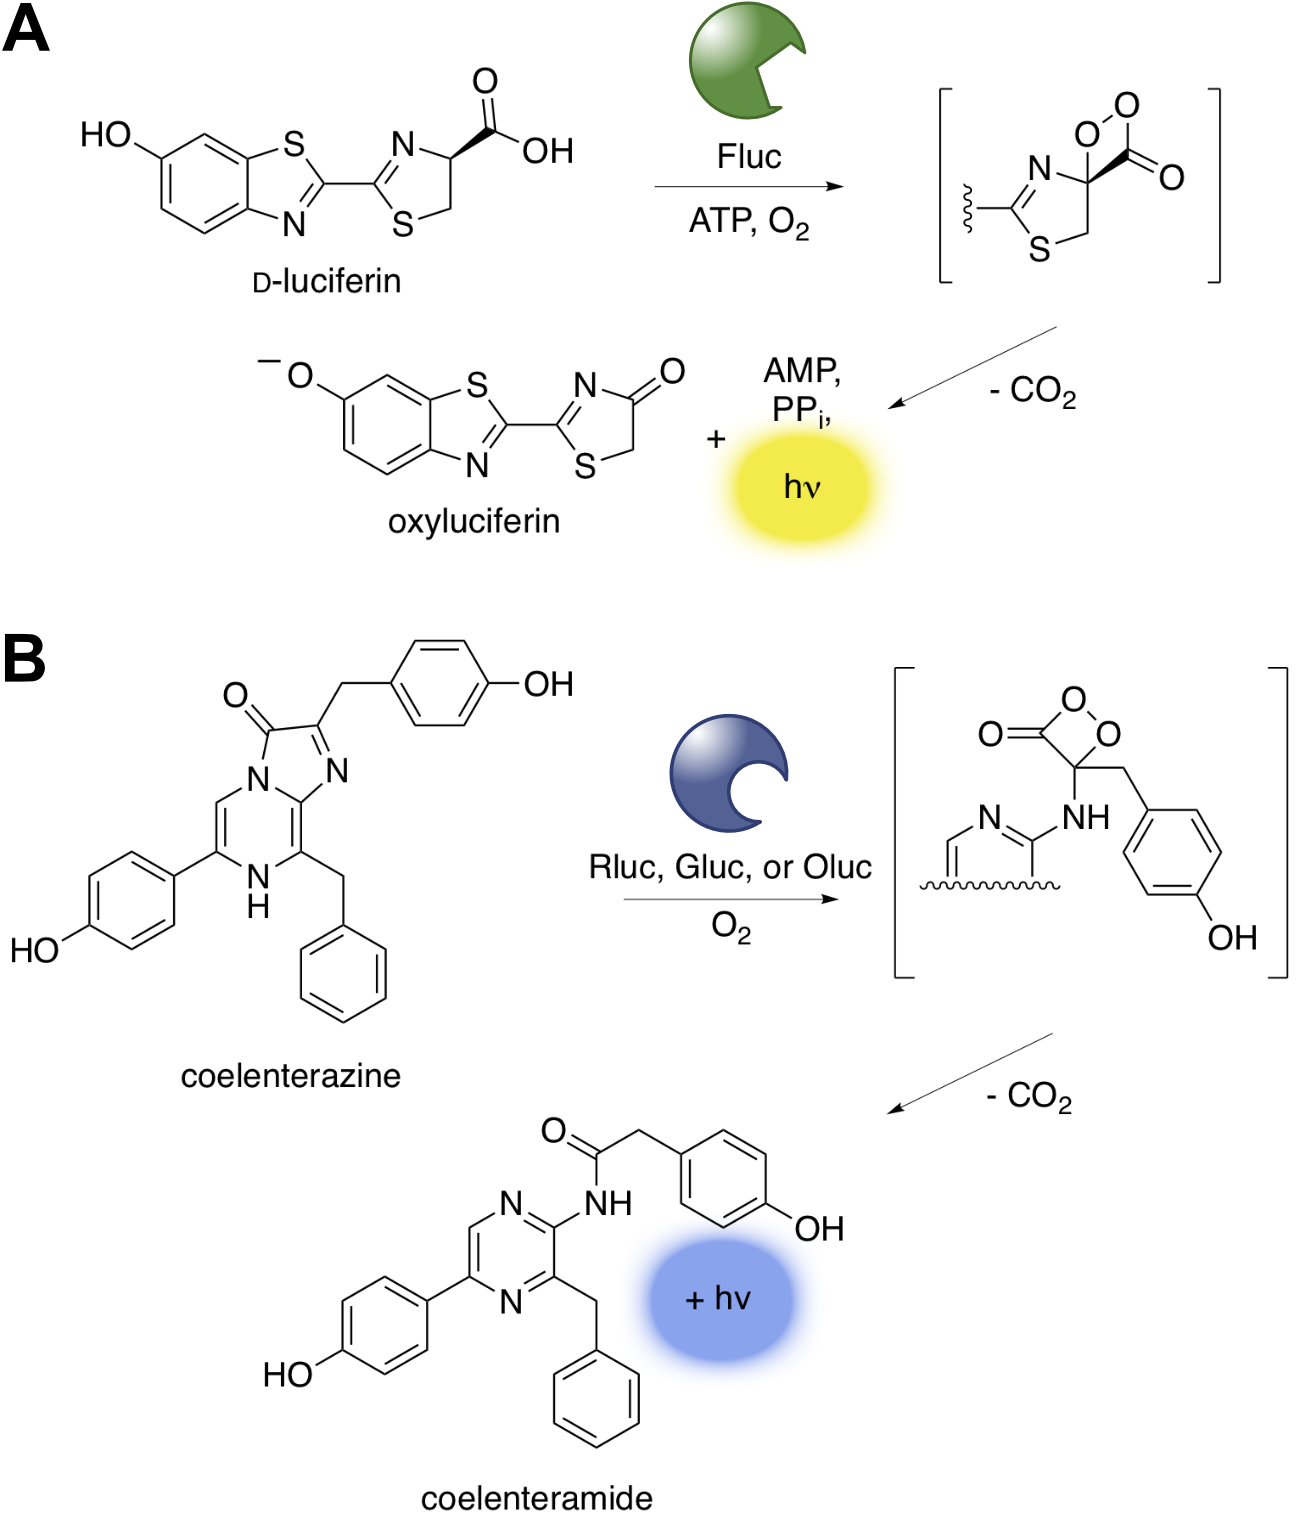
\includegraphics[width=85 mm]{chapter1/figure1_2}
\centering
\caption[Popular luciferase-luciferin pairs for cellular imaging]{Popular luciferase-luciferin pairs for cellular imaging. (A) DLuciferin
is oxidized by firefly luciferase (Fluc) to produce oxyluciferin
and a photon of light. (B) Coelenterazine is oxidized by a variety of
marine luciferases, including Renilla luciferase (Rluc), Gaussia
luciferase (Gluc), and Oplophorus luciferase (Oluc). These luciferases,
unlike Fluc, require only oxygen as a cofactor in the light-emitting
reaction.}
  \label{fig:luc_oxidation}
\end{figure}

Despite their distinct chemical
structures, D-luciferin and coelenterazine use a similar
mechanism for light production: the cognate luciferases oxidize
the small molecules to generate excited state oxyluciferins;
relaxation of these molecules to the ground state results in
photon emission (Figure \ref{fig:luc_oxidation}).
The color of light released is primarily dictated by the small
molecule luciferin. In the case of D-luciferin, the aromatic core
is sufficiently extended to provide yellow-green ($\approx$560 nm)
light. For coelenterazine, the $\pi$ system of the putative emitter is
shorter, resulting in blue wavelengths ($\approx$475 nm) of emission.
The luciferase environment can further modulate bioluminescent
color. Thus, enzymes that use the exact same substrate can
emit different wavelengths. In some cases, the emission spectra
are sufficiently resolved to enable multicolor imaging.\cite{Suzuki:2016jw}
Discriminating among related luciferases in vivo, though,
remains difficult because of their broad emission spectra and
the strong absorption of $>$650 nm light.\cite{Zhao:2005if}
\section{Building better bioluminescent tools}
Luciferases and luciferins have been used for decades to image
biomolecules, gene expression, and even whole cells, but the
most popular probes are not without limitation.\cite{RN26} The poor
tissue penetrance of many luciferins has historically precluded
sensitive imaging in hard-to-access tissues (e.g., brain).
Additionally, only a limited palette of bioluminescent probes
exists, hindering efforts to visualize multicellular or other
multicomponent processes. Chemical and biological approaches
are beginning to address the need for improved and
more diverse collections of bioluminescent probes.
\subsection*{Streamlined and Scalable Luciferin Syntheses} 
Most bioluminescence imaging studies require an exogenously
delivered luciferin. For in vivo work, the doses can range
between 1 and 5 mg per mouse per imaging point. Thus,
large--and often prohibitively expensive--quantities of luciferin
are required for animal studies. Accessing luciferins in bulk
has been a historic challenge. The chemical complexity of Dluciferin
and coelenterazine has also frustrated efforts to rapidly
diversify these scaffolds to produce new analogues.
In recent years, improved methods for producing luciferins
have been reported. In the case of D-luciferin, we developed a
streamlined method for accessing the requisite benzothiazole
core using Appel's salt and modern C-H activation (Figure \ref{fig:luc_derivatives}).\cite{McCutcheon:2012ixb} 

\begin{figure}[htbp]

\includegraphics[width= 85 mm]{chapter1/figure2_v3}
\centering
\caption[Recently synthesized luciferin heterocycles]{Recently synthesized luciferin heterocycles. (A) D-Luciferin
and related analogues can be accessed using Appel's salt and C-H
activation chemistry. (B) A diverse array of coelenterazine analogues
have been synthesized in recent years.}
  \label{fig:luc_derivatives}
\end{figure}

This approach improved the yield and generalizability of
the synthesis, eliminating the need for multiple functional
group conversions used in previous routes. The strategy has
enabled multigram syntheses of D-luciferin and has proven to
be quite modular. In fact, we and others have used this
chemistry to produce more than 30 distinct analogues.\cite{Woodroofe:2012vx} Many
of these scaffolds also comprise key functional handles for late stage
diversification (Figure \ref{fig:luc_derivatives}). Efforts to expediently
synthesize amino luciferins\cite{Hauser:2016jt} and related analogues\cite{Anderson:2017hb} are similarly
facilitating more widespread use of bioluminescent tools.
Improved methods for accessing coelenterazine analogues
are also advancing imaging studies. Historically, coelenterazine
synthesis relied on condensation of glyoxal derivatives with
strong acid and elevated temperatures. These conditions are
incompatible with a diverse array of desired analogues. Kirkland
and colleagues identified milder conditions to access the
coelenterazine core via Horner-Wadsworth-Emmons olefination.\cite{Shakhmin:2016bd}
The method proved to be both scalable and generalizable,
providing a range of useful analogues. Recent advances
in cross-coupling methodology are similarly enabling access to
diverse coelenterazine architectures.\cite{Hosoya:2015iu}
\subsection*{Brighter and More Colorful Probes}
Bioluminescence imaging to date has been largely confined to imaging one or
two colors at a time. Accessing a full spectrum of emitters has
been a long-standing goal, with obvious parallels to
fluorescence imaging. Early efforts to modulate color and
brightness primarily focused on the luciferase enzyme.\cite{RN26} Recent
years, though, have seen a shift in focus to modulating the small
molecule (Figure \ref{fig:luc_spectrum}).

\begin{figure}[htbp]
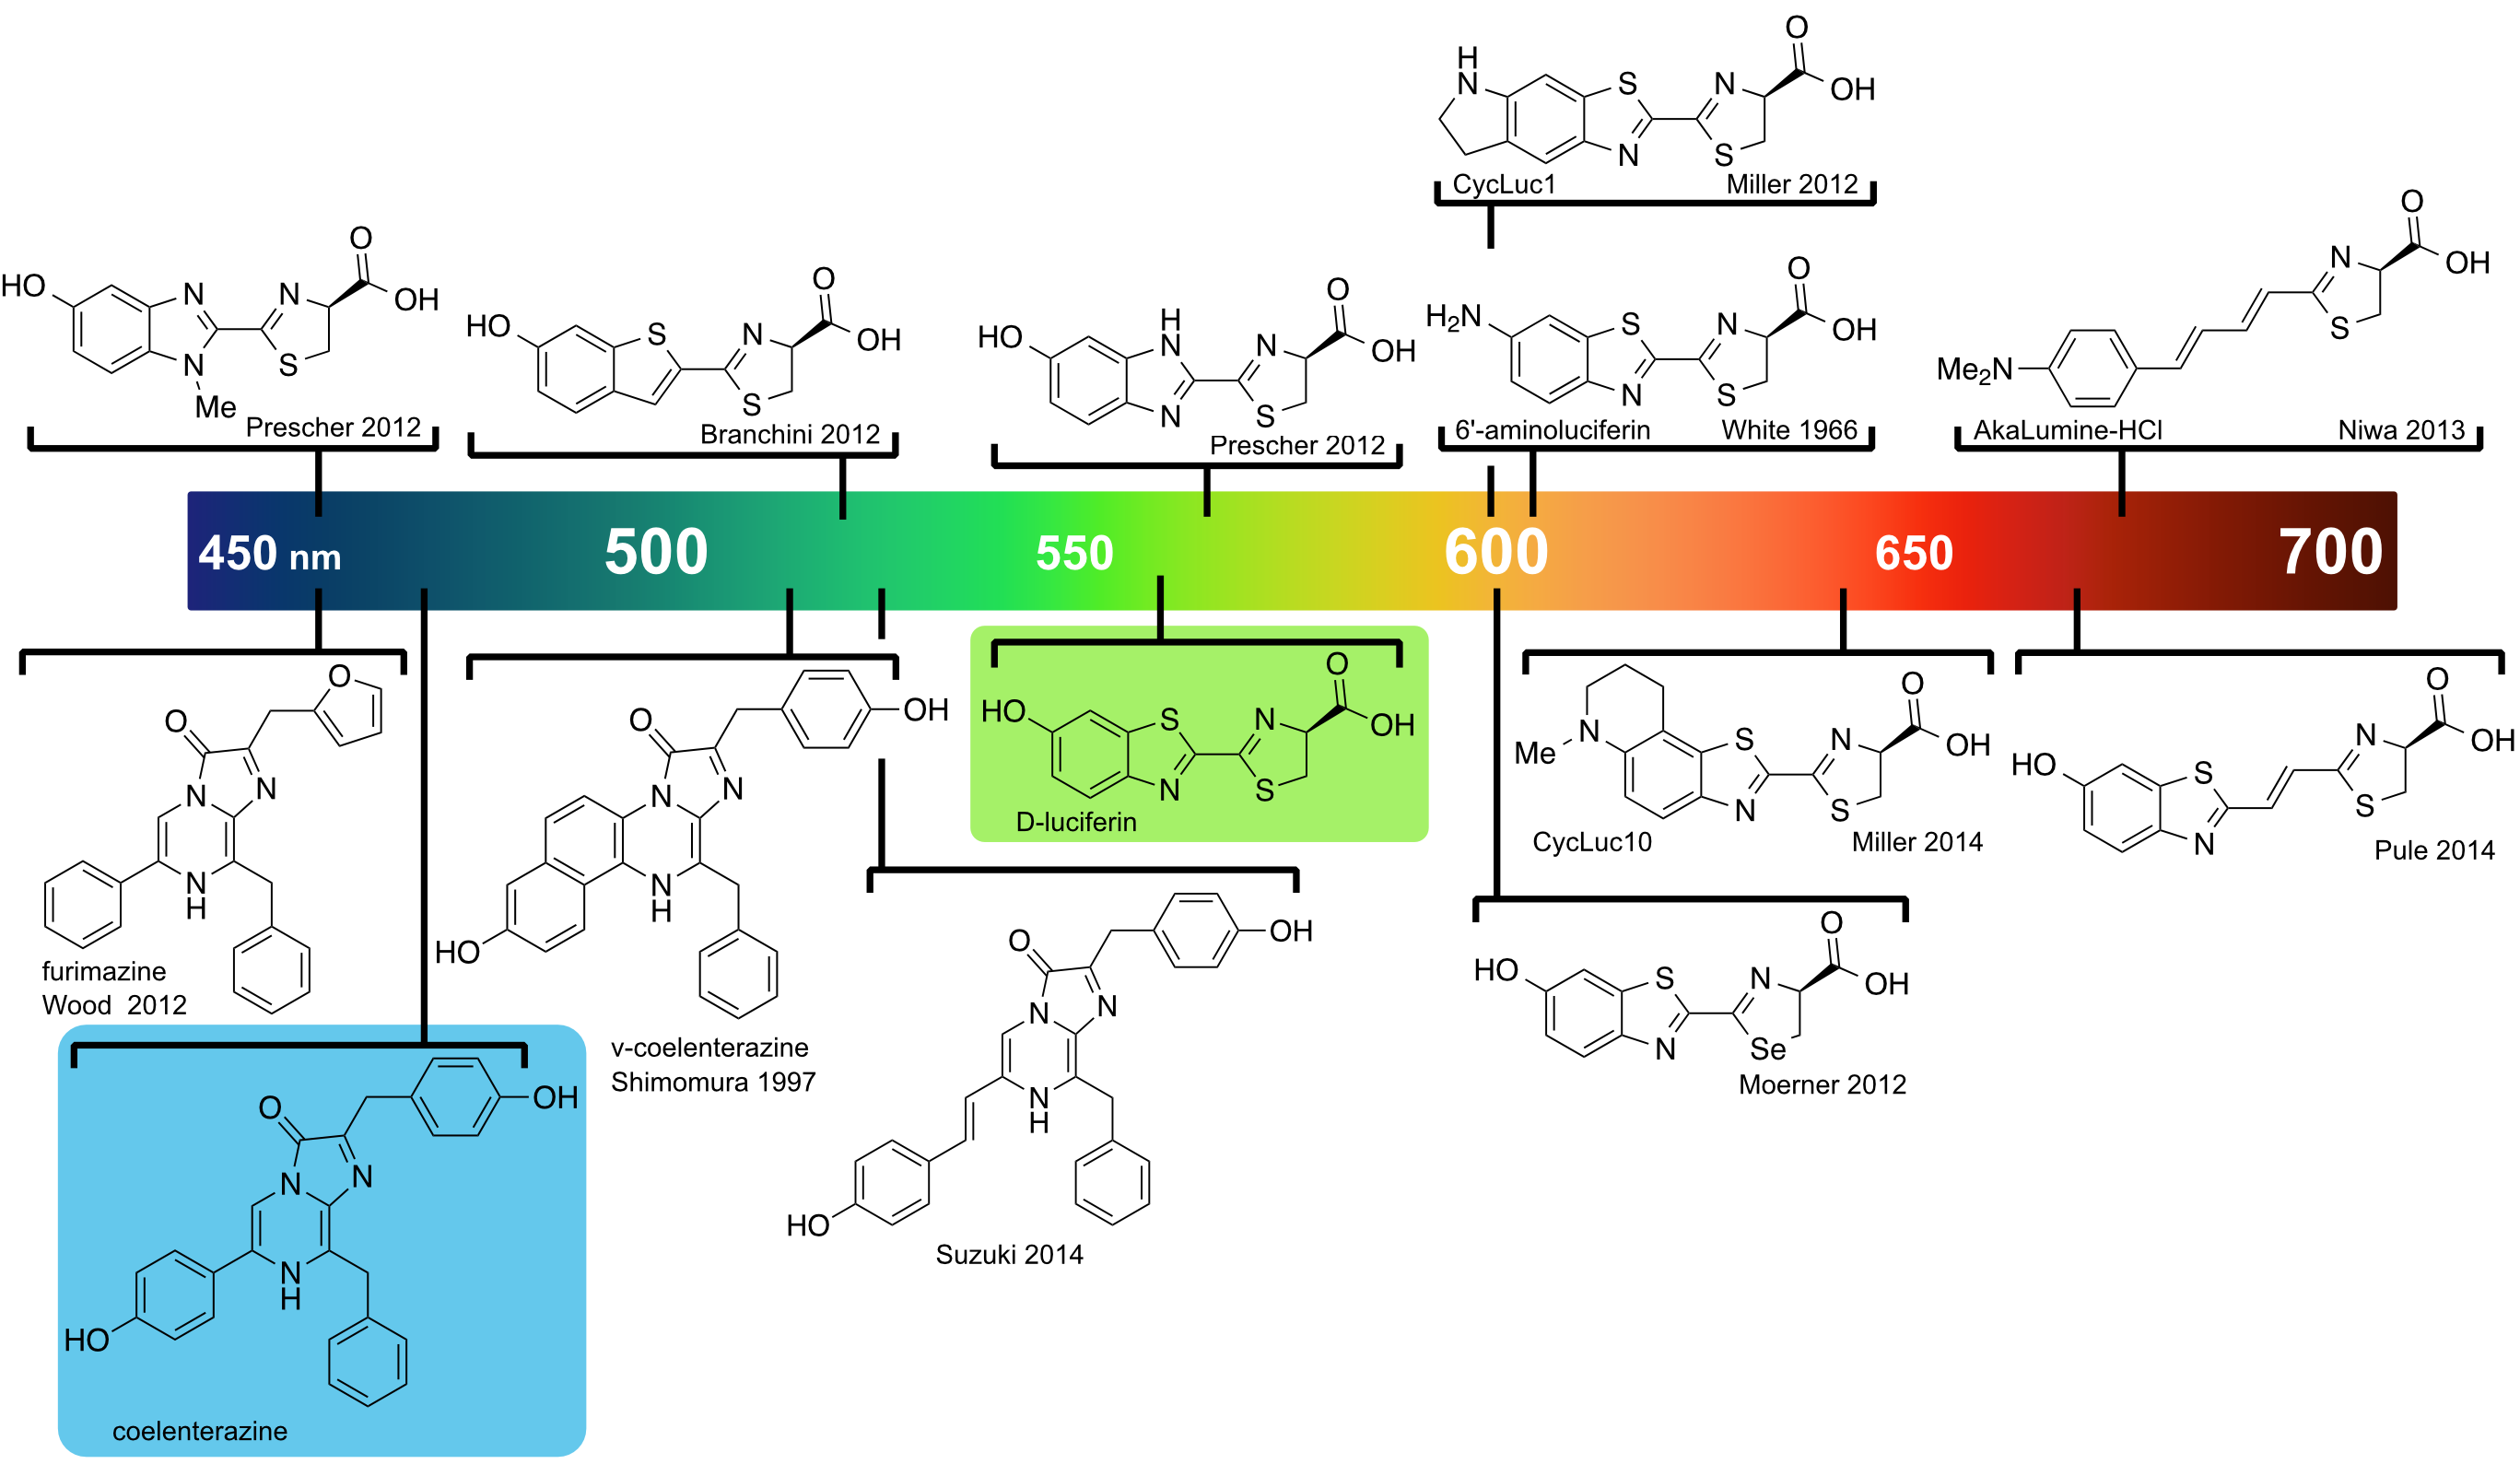
\includegraphics[width= \textwidth]{chapter1/spectrum_revision}
\centering
\caption[Palette of luciferin analogues]{Palette of luciferin analogues. Native luciferins are highlighted with colored boxes. Brackets denote the wavelength (nanometers) of
maximal bioluminescence emission observed upon incubation of the compound with luciferase. While many analogues can provide unique colors of
light, most are not efficiently processed by native luciferases.}
  \label{fig:luc_spectrum}
\end{figure}

Because the structure of the luciferin emitter influences
bioluminescent output, methods for modulating color and
intensity often parallel those in small molecule fluorophore
development. For example, rigidifying the aromatic core can
provide improved push-pull chromophores and enhanced
light emission. Miller and coworkers applied this strategy to Dluciferin,
replacing the rotationally flexible 6' electron-donating
group with a conformationally locked amine.\cite{Reddy:2010gaa} This configuration
enabled enhanced donation of electrons to the luciferin
core and more robust, red-shifted emission compared to that of
related probes.\cite{Chu:2016im} Moreover, many of the cyclic luciferin (CycLuc)
scaffolds were viable substrates for Fluc, highlighting the
promiscuity of the enzyme.
Fluc can also process luciferin analogues with extended
aromatic cores and modified heteroatoms, providing additional
avenues for wavelength alteration.\cite{McCutcheon:2012ixb,Woodroofe:2012vx,RN100} $\pi$-Extended chromophores
typically emit red-shifted light emission.\cite{Kuchimaru:2016eba} In the case of
the vinyl-extended luciferins (Figure \ref{fig:luc_spectrum}), the shift was $>$100 nm.
It should be noted, though, that these and other extended
analogues are often poorly processed by Fluc itself; red-shifted
emission comes at the expense of enzyme turnover and thus
total photon output.
Parallel developments in coelenterazine synthesis have
provided scaffolds that emit different colors of light. Redshifted
probes are particularly desirable for imaging with Rluc
and Gluc in vivo, as the normal blue emission with these
enzymes is strongly absorbed by blood.\cite{Zhao:2005if} Inouye and colleagues
recently developed a streamlined synthesis of a conformationally
locked coelenterazine for improved imaging.\cite{Hosoya:2015iu} Others have
explored luminophores with extended $\pi$-conjugation to achieve
more tissue-penetrant wavelengths of light.\cite{Nishihara:2014cr,Grinstead:2016gh}
Bioluminescent color and photon output can also be
drastically modulated via bioluminescent resonance energy
transfer (BRET). A recent fusion of NanoLuc (an optimized
mutant luciferase, discussed below) to CyOFP1 [dubbed
Antares (Figure \ref{fig:antares}A)] resulted in an emission shift of 114 nm
(Figure \ref{fig:antares}B).\cite{Chu:2016im} 

\begin{figure}[htbp]
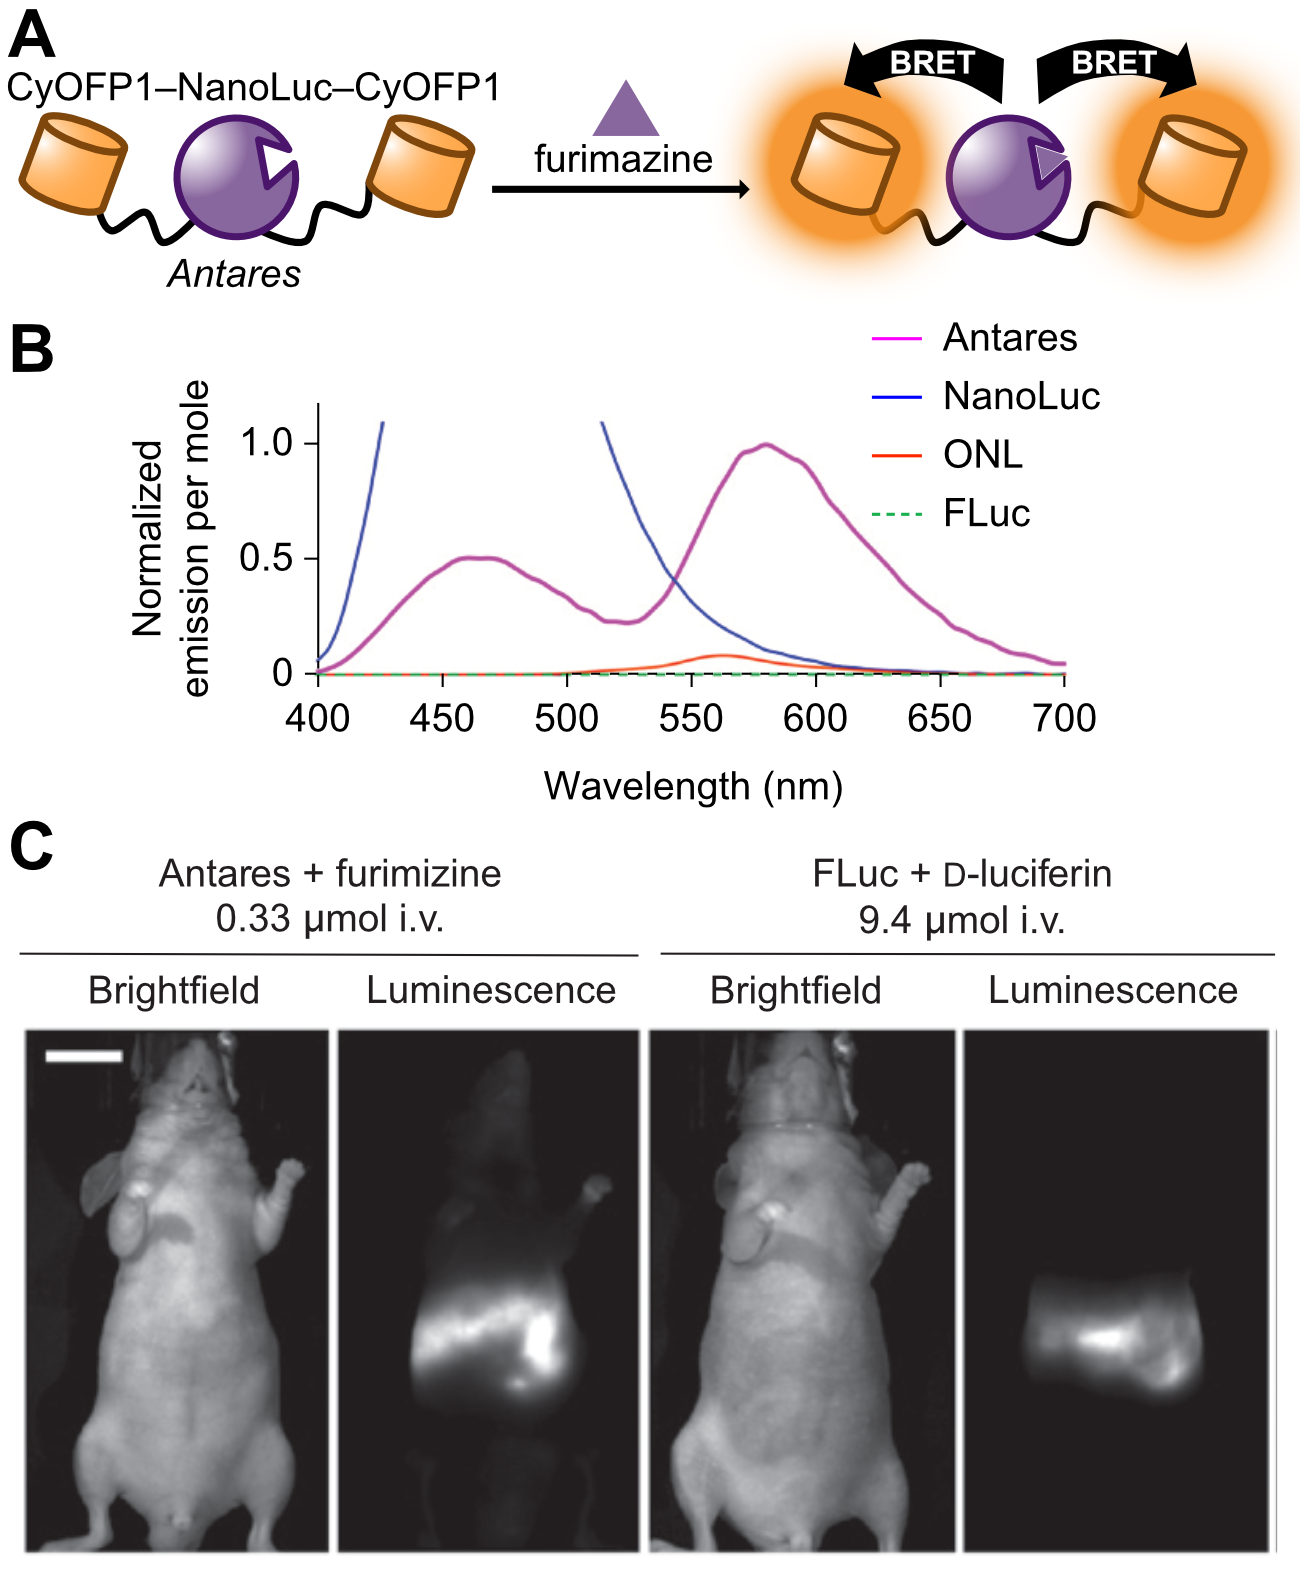
\includegraphics[width= 85 mm]{chapter1/antares_2}
\centering
\caption[BRET for deep-tissue imaging]{BRET for deep-tissue imaging. (A) Antares comprises a
fusion of NanoLuc with two cyan-excitable orange fluorescent proteins
(CyOFP1). (B) The BRET fusion exhibits red-shifted emission
relative to NanoLuc. ONL denotes Orange Nanolantern. (C) Antares enabled
sensitive imaging with low luciferin levels in mice. Antares and
Fluc genes were delivered to the liver via hydrodynamic injection.
Luciferins were supplied intravenously. Adapted with permission from
ref \cite{Chu:2016im}.}
  \label{fig:antares}
\end{figure}

Antares is one of the most red-shifted BRET
pairs reported to date, enabling enhanced deep-tissue imaging
in vivo (Figure \ref{fig:antares}C). In related work, Nagai and colleagues
linked a mutant Renilla luciferase to Venus, a version of yellow
fluorescent protein.\cite{Saito:2012gs} Unexpectedly, this construct (dubbed
Nanolantern) produced 6-fold more photons than the
luciferase alone and shifted emission into the yellow-green
region (530 nm). Additional Nanolantern colors have been
described.\cite{Suzuki:2016jw} Collectively, these and other BRET probes are
enabling sensitive imaging of many biological processes,
including membrane voltage\cite{Inagaki:2017kj} and gene expression.\cite{Horikiri:2017bt}
\subsection*{In Vivo Improvements}
Luciferins can access most tissues, but their distribution and cell permeability are suboptimal and
not uniform.\cite{RN101} Chemical tinkering and med-chem optimization
can improve the bioavailabilities of the substrates. For example,
many of the CycLuc scaffolds that comprise more lipophilic
amino modifications (vs -OH groups) exhibit improved tissue
penetrance in vivo.\cite{RN98} Far less compound is required for a given
imaging session compared to native luciferins. Further
amidation of a CycLuc probe enhanced its transport across
the blood?brain barrier (Figure 5).\cite{Mofford:2015br} Once the probe is in the
brain, the amide bond can be cleaved by endogenous fatty acid
amide hydrolase (strongly expressed in brain tissue), releasing a
functional luciferin.
\section{Luciferase-luciferin pairs for multicellular imaging}
Many improvements to the luciferin small molecules noted
above came at the expense of luciferase turnover (and thus light
output). Consequently, recent efforts to build improved
bioluminescence tools have focused on identifying new
substrates and enzymes in parallel. One source of new
luciferase-luciferin pairs is nature itself. Bioluminescent
organisms (and potentially new luciferase-luciferin pairs) are
continually being described,\cite{Purtov:2015hx} though the need for optimized
probes far outpaces their discovery. Others have turned to
engineering existing luciferases to better use chemically
modified luciferins. In one example, Miller identified mutant
luciferases that can more readily process CycLuc derivatives.
These analogues were previously demonstrated to be viable
substrates for Fluc, although oxyluciferin products inhibited the
reaction. Substrate inhibition was relieved and long-lived light
emission restored with mutant enzymes.\cite{Harwood:2011gl} The authors later
identified a mutant that preferred a luciferin analogue over Dluciferin,
setting the stage for developing substrate-responsive
enzymes.\cite{RN97} Further work by the Miller group revealed latent
luciferase activity in a fatty acyl-CoA synthetase from the
fruitfly.\cite{RN165} Interestingly, this enzyme did not emit light with Dluciferin--it
was able to use only a CycLuc substrate--opening
the door to pairing unnatural luciferin analogues with
evolutionary relatives of luciferase.
Another engineered bioluminescent enzyme that has seen
widespread adoption in recent years is NanoLuc, a derivative of
Oplophorus luciferase (Oluc).\cite{Hall:2012cda} Early work in this area was
motivated by the need for improved coelenterazines (molecules
prone to autoxidation and exhibiting poor tissue penetrance)
and Oluc subunits (enzyme fragments prone to instability).
Seeking a brighter and more stable luciferin, Wood and
colleagues replaced the electron-rich phenols of coelenterazine
with phenyl and furan groups. The resulting molecule
[furimazine (Figure \ref{fig:luc_spectrum})] was more stable in media and lysate
and less susceptible to nonspecific oxidation. Directed
evolution was used to select an enzyme that could readily
catalyze light emission from the designer luciferin. The
winning mutant (NanoLuc) contained a total of 16
mutations, an impressive number for a 16 kDa protein.
NanoLuc exhibits a high turnover rate with furimazine,
providing robust signal output. Such high photon flux values
are enabling sensitive imaging in complex tissue samples, even
point-of-care diagnostics with simple cell phone cameras.\cite{Griss:2014de} We
anticipate that the popularity of the NanoLuc-furimazine pair
will continue to surge in the near term.

Tandem modification of bioluminescent enzymes and
substrates is also enabling multicomponent bioluminescence
imaging. In contrast to in vitro assays, imaging in vivo often
precludes spectroscopic resolution of colored probes. Blood
and tissue restrict the passage of wavelengths shorter than red,\cite{Zhao:2005if}
and bioluminescence spectra are broad,\cite{Rumyantsev:2016fd} necessitating an
alternative approach. Substrate resolution is one such strategy
(Figure \ref{fig:jacs_summary}A). 

\begin{figure}[htbp]
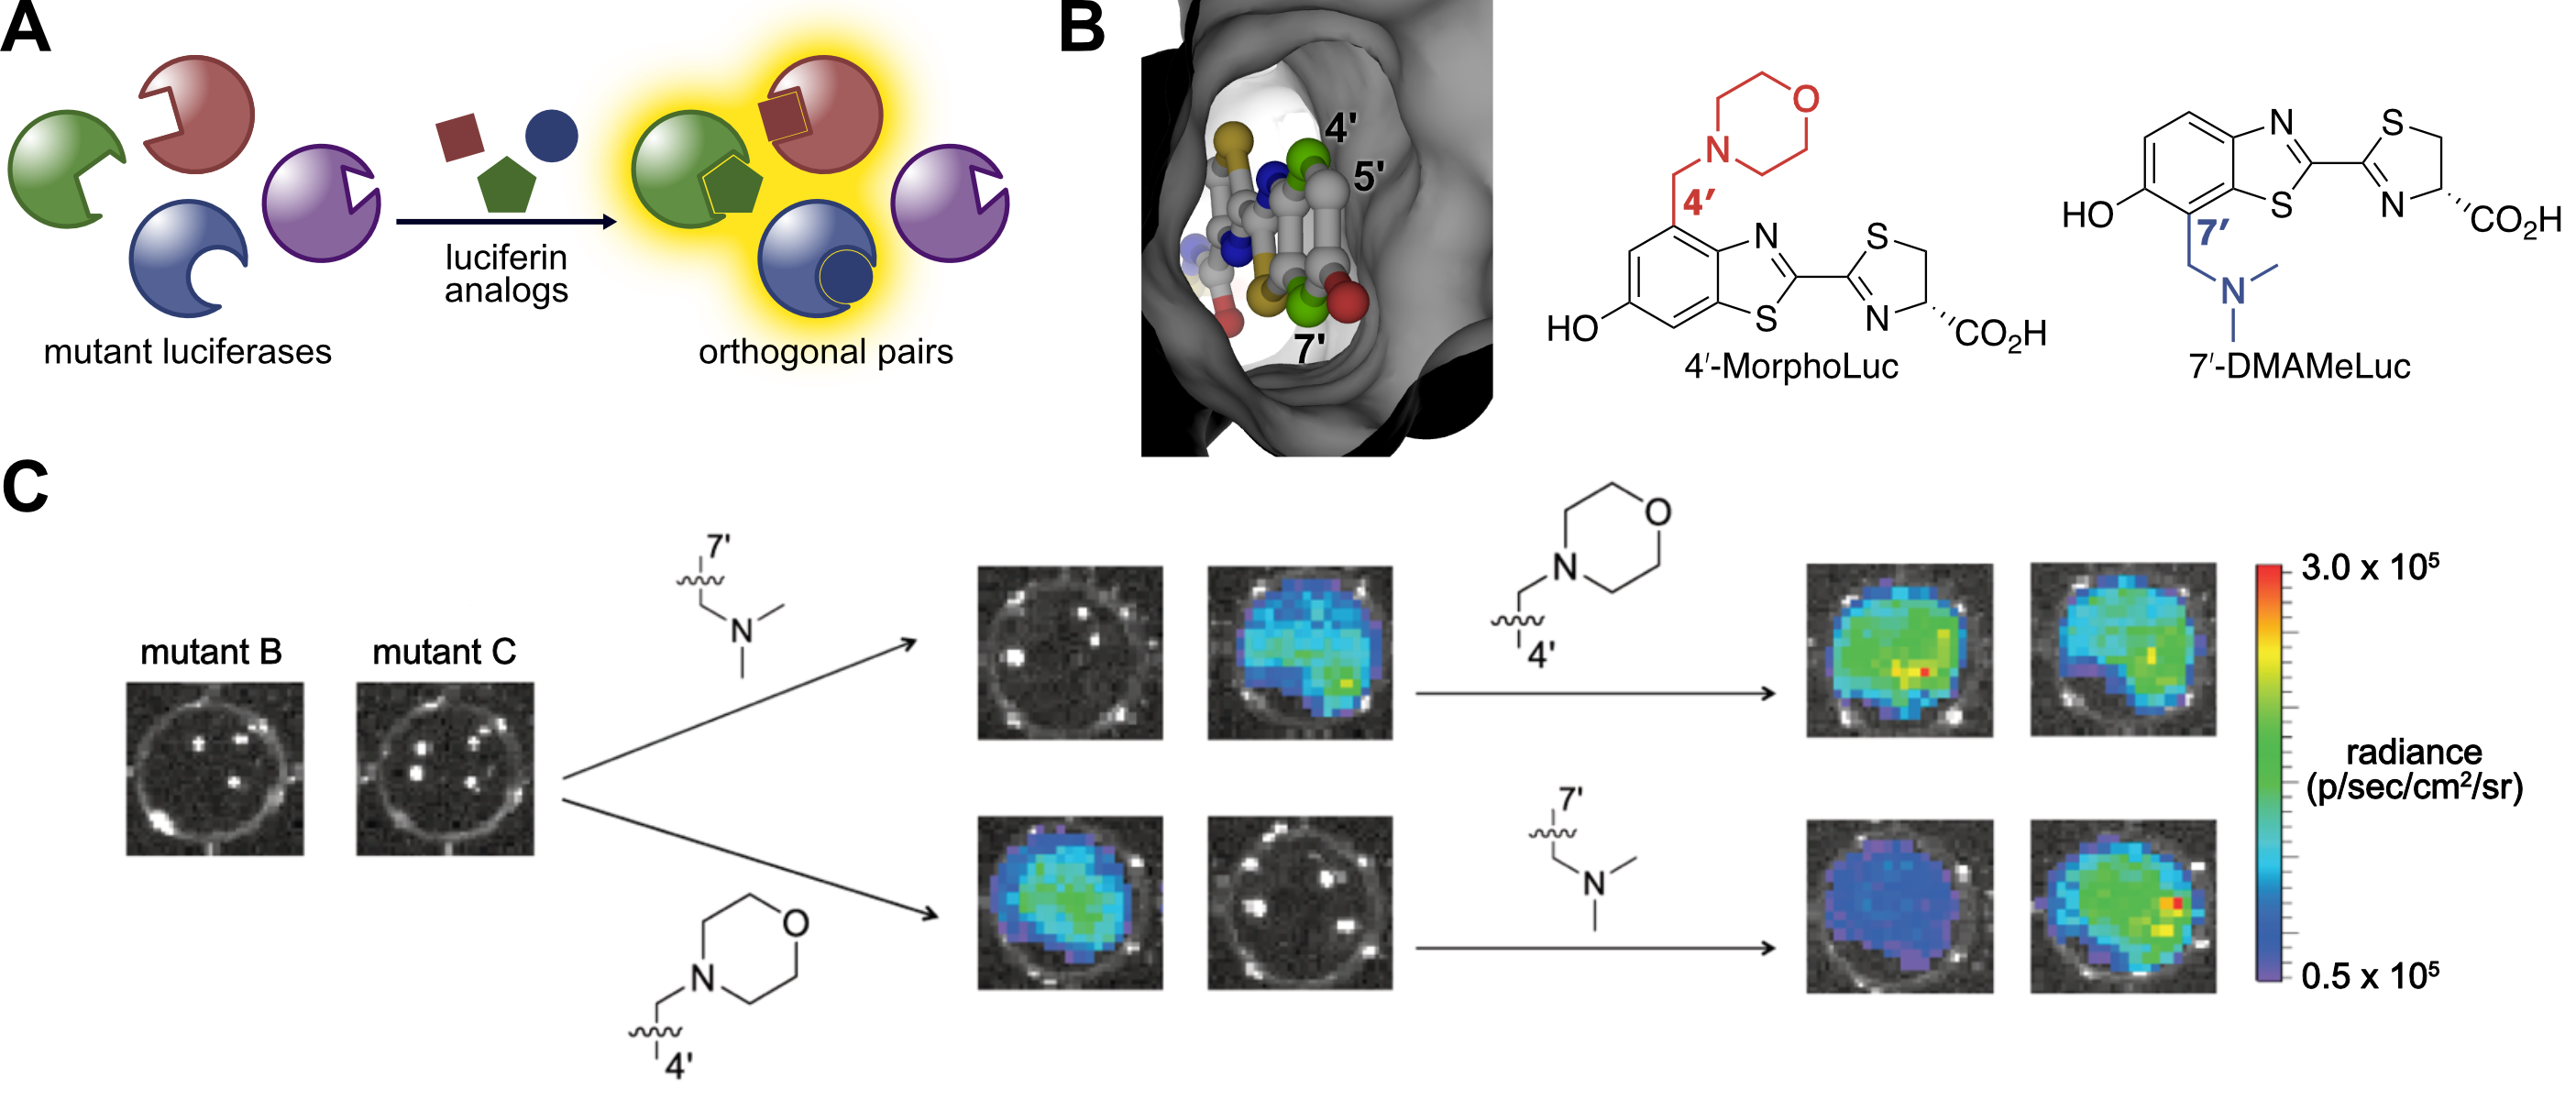
\includegraphics[width= \textwidth]{chapter1/figure6}
\centering
\caption[Orthogonal luciferin-luciferase pairs for multicomponent imaging]{Orthogonal luciferin-luciferase pairs for multicomponent imaging. (A) A strategy for multicomponent bioluminescence imaging with
luciferin analogues and mutant luciferases. (B) The 4? and 7? sites of D-luciferin were targeted to preclude binding to native Fluc. (C) Substrate
resolution was achieved in mouse DB7 cells using 4?- and 7?-modified luciferins and mutant luciferases identified from screening. Adapted with
permission from ref \cite{Jones:2017be}.}
  \label{fig:jacs_summary}
\end{figure}

This approach requires multiple selective,
mutually orthogonal luciferin-luciferase pairs. These pairs
produce light together but will not react with other mutants or
enzymes. Orthogonal pairs already exist in nature (e.g., firefly
and marine luciferases, along with their requisite substrates),
and many have been adapted for dual-imaging studies.
To expand and expedite the search for orthogonal pairs,30 we
turned to producing non-natural analogues and enzymes. We
synthesized a panel of luciferins, with additional steric bulk at
the 4? and 7? positions (Figure 6B). We screened these
analogues against libraries of luciferase mutants to produce
more than 3000 potential pairings. To find substrate-resolved
hits in this milieu, we mined the data with a computer
algorithm. This strategy revealed two enzymes that exhibited
substrate resolution with two compounds (one 4' and one 7').
This pair proved to be successful in mammalian cells, as well,
demonstrating the robust nature of our screening methodology
(Figure 6C). In an analogous approach, Kim and colleagues
recently reported substrate-resolved bioluminescence imaging
with coelenterazine analogues.32
\section{Bioluminescent reporters for cell--cell interactions}
A second challenge being addressed by improved bioluminescent
tools is monitoring cellular interactions in vivo.
Conventional bioluminescence imaging can detect small
numbers of cells, but historically has lacked the spatial
resolution to precisely pinpoint their locations or interactions
in whole organisms. Target recognition and cell?cell contacts
are crucial to numerous physiological processes, including
neurotransmission, immune function, and cell migration, so
methods to globally assay such interactions are necessary.
The development of tools that report on cell?cell contacts
has been inspired by classic methods for reporting on
biomolecule activities and interactions. For example, caged
probes have been used widely to report on small molecule
analytes in cells. We and others33 have shown that such cages
can be repurposed to image interactions between cells (Figure
7A). In a recent example, a ?dark? luciferin comprising a 6?-
nitro group (Luntr) was used as the cage.34 This probe could
be reduced by one group of cells (expressing nitroreductase)
and used by a neighboring group of cells expressing luciferase.
Light emission was strongest in areas of cellular contact.
Nitroreductase is not expressed endogenously in mammalian
cells, making this technology ripe for in vivo applications where
high spatial sensitivity is required.

A second class of cell contact sensors uses split reporters,
originally developed to image protein?protein interactions
(Figure 7B). We expanded on this concept to generate split
reporters of cell proximity using Gaussia luciferase (Gluc), a
secreted protein that functions in the extracellular space. Split
fragments of Gluc were fused to leucine zippers Fos and Jun to
drive complementation. The N-terminal half was expressed in
one cell population and the C-terminal half in another. Light
emission in this case tracked with distance between the cell
populations (Figure 7C).
\section{Bioluminescent reporters for analyte detection in vivo}
Bioluminescence has long been exploited for detecting enzyme
activities and low-abundance metabolites. The majority of these
studies, though, have been limited to ex vivo analyses with
cultured cells or excised tissues. Continued advances in
bioluminescence technology are enabling new probes to be
applied as biosensors in vivo.36,37 In a recent example, Chang
and colleagues developed a copper ion sensor for imaging in
mice. The probe comprised a caged luciferin, with a bulky
chelator group (i.e., the ?cage?) attached to the 6? position of Dluciferin.
The sterically encumbered molecule was poorly
utilized by luciferase. Upon removal of the cage by copper-
(I)-dependent oxidative cleavage, a viable luciferin was liberated
and available for light emission. Photon production could thus
be correlated to copper ion levels. The caged probe was
ultimately used for analyte imaging in mouse models of fatty
liver disease.36
\section{Conclusions and future directions}
Bioluminescence has historically lagged behind fluorescence
imaging in terms of the breadth and diversity of available tools.
Recent advances in luciferin chemistry and luciferase engineering,
though, are beginning to fill this gap. New synthetic
methods are providing novel luciferin architectures for
improved imaging. Engineered luciferases are enabling the
sensitive detection of cells and other analytes in vivo.
Combinations of designer substrates and mutant enzymes are
furthering the range of potential applications. It is now possible
to image multicellular features in live animals, visualize cells in
difficult-to-access tissues (e.g., brain tissue), and selectively
illuminate cell?cell interactions. Moving forward, we anticipate
continued advances in red-shifted probes, tandem luciferase?
luciferin engineering, and sensors for cellular metabolites.
These tools will influence how researchers conduct experiments
involving multiple cell types and molecular features beyond the
culture dish. Additionally, like other useful imaging agents, the
tools will likely facilitate discoveries in a diverse range of fields.

%%% Local Variables: ***
%%% mode: latex ***
%%% TeX-master: "thesis.tex" ***
%%% End: ***
